\documentclass[a4paper,10.0pt,twoside]{npr}

\usepackage{multicol,graphicx,lastpage,footmisc,fancyhdr,paralist,
tabularx,array,booktabs,caption,multirow,upgreek,mathrsfs,gensymb,color}
\usepackage[fancyhdr,space,fntef,fontset=ubuntu]{ctex}
\usepackage{amssymb,bm,mathrsfs,bbm,amscd}
\usepackage{flushend,cuted}
\usepackage{refcount}
\usepackage{savesym}
\usepackage{textcomp}
\usepackage[tbtags]{amsmath}  %
\savesymbol{iint}
\usepackage{amstext} %数学宏包文本命令
\usepackage{balance} %版心底部对齐

\flushbottom      %版心底部对齐
\setcounter{section}{0}
\begin{document}
%\begin{CJK*}{GBK}{\song}{\wuhao}{\rm}

%___________________________________________________________________________________
\def\rd{{\rm d}}

\newcommand{\RM}{\ensuremath{\mathrm}}   %正体 既可用于文本模式也可用于数学模式
\newcommand{\dif}{\mathrm{d}}  %直立体d
\newcommand{\me}{\mathrm{e}}  %直立体e
\newcommand{\mi}{\mathrm{i}}  %直立体i
\newcommand{\mj}{\mathrm{j}}  %直立体j
\newcommand{\afrac}[2]{\dfrac{\,#1\,}{\,#2\,}}  %略长分数线
\newcommand{\nn}{\nonumber}  %公式无编号
\newcommand{\nt}{\noindent}
\newcommand{\OO}{~\text{。}}
\newcommand{\PP}{~\text{,}}
\newcommand{\OP}{~\text{;}}
\newcommand{\LT}{\left}
\newcommand{\RT}{\right}

%___________________________________________________________________________________

\balance
\fancypagestyle{myfoot}
{%
\fancyhf{}
\fancyhead[c]{\wuhao\song 高~等~核~物~理~实~验}
\renewcommand{\headrule}{\vskip 2pt
\hrule height0.4pt width\headwidth \vskip1pt
\hrule height0.4pt width\headwidth \vskip-1.8pt}
}%
\thispagestyle{myfoot}

%%%%%%%%%%%%%%%%%%%%%%%%%%%%%%%%%%%%%%%%%%%%%%%%%%%%%
%    奇偶页眉
%%%%%%%%%%%%%%%%%%%%%%%%%%%%%%%%%%%%%%%%%%%%%%%%%%%%%
\pagestyle{fancy}
\fancyhead{}
\fancyhead[ce]{\xiaowu\song \hspace{0.5em}高~等~核~物~理~实~验}
%\fancyhead[ro,le]{\xiaowuhao \hspace{0.5em}\textbf{\textperiodcentered}\;\thepage\;\textbf{\textperiodcentered}\hspace{0.5em}}
%\fancyhead[ce]{\xiaowu\song 粒~子~物~理~与~原~子~核~物~理~专~题~实~验}
%\fancyhead[re]{\xiaowu\song \hspace{0.5em}第\;31\;卷\hspace{0.5em}}
\fancyfoot[ce,co]{}
\renewcommand{\headrule}{\vskip 2pt
\hrule height0.4pt width\headwidth}


\setcounter{page}{001}%
\fancyhead[co]{\xiaowuhao\song  乔颢:CsI(Tl)闪烁体能量分辨率的研究}    %奇页页眉
\begin{center}
\title{%
\xiaoerhao \bf  %章标题为两行时改为 \exiaoer
CsI(Tl)闪烁体能量分辨率的研究\\[-5mm]}
\maketitle
\large \fs
乔颢$^{^1}$\\[2mm]

\xiaowu \song
1. 北京大学物理学院,海淀区 北京 100871;\\[4mm]

 
\footnotetext[0]{{\bf 作者简介:}~~\begin{minipage}[t][4.2mm]{149mm}\song
乔颢,E-mail: i@catofes.com
\end{minipage} }
%\footnotetext[0]{{\bf 通信作者:}\song ~~E-mail: xxx@xxx.xxx }%通信作者为第一作者时不要此项

\parbox{158mm} {
\zywu{\bf 摘要:}~~\fs
该实验使用CsI(Tl)闪烁体和光电倍增管耦合制作探测器,测量Cs的全能谱。得到探测器的能量分辨率为16\%。
\\
{\bf 关键词:}~~\fs CsI闪烁体,耦合,能量分辨率}\\
\end{center}
%%%%6.正文
\vspace{5mm}
%%%%6.正文
\setcounter{section}{0}
\begin{multicols}{2}
%----------------
%_________三__________________________________________________小_________________
%%%%以上请不要改动%%%%%%%%%%%%%%%%%%%%%%%%%%%%%%%%%%%%%%%%%%%

\section{引言}    %1
\vspace*{-1mm}
\song\wuhao

闪烁体探测器是测量辐射粒子能量的一种重要方法,通过探测入射粒子的特征能量来分辨粒子的种类。当粒子入射到闪烁体内部后,与闪烁体相互作用发光,而后被光电倍增管接受放大输出电信号。因为其了可以探测的粒子种类多,探测效率高,能够探测能量和强度,因此在核物理实验中有着及其广泛的应用。
本实验中通过闪烁体探测器影响能量分辨率的种种因素,在教学实验的条件下尽量提高入射粒子的能量分辨率,为以后的研究奠定基础。

\section{实验}
\subsection{实验介绍及原理}
闪烁体探测器是利用某些物质在射线的作用下会发光的特性来探测射线的仪器。本试验中的探测器属于信号性探测器,主要用于测量辐射粒子的强度和能谱。本实验中使用的闪烁体是CsI(Tl)无机闪烁体,是使用铊作为激发剂的碘化铯闪烁体。

影响能量分辨率的因素主要有以下几个方面,首先是闪烁体的包装。因为闪烁体中间激发的光子是发散到各种方向的,因而为了减少因为散射造成的损失,要用反射率高的材料对闪烁体进行包装。包装材料和包装的合适程度都会影响闪烁体的性能。因为闪烁体的折射率是大于空气的,因此在闪烁体和光电倍增管之间要用折射率高的材料进行耦合,一般是使用硅脂或者硅油。经过闪烁体后信号就会进入到电子学部分,而电子学部分对于整体实验能量分辨率的影响也至关重要。

\subsection{实验过程和步骤}

首先使用tyvek包装纸包装闪烁体,包装纸至少包两层,完全覆盖闪烁体以提高分辨率。随后使用黑色的遮光材料覆盖闪烁体,避免外部的光进入闪烁体。

然后将闪烁体与光电倍增管进行耦合。耦合的作用是避免闪烁体和广电倍增管之间因为有气隙从而发生全反射。因此需要多碾磨几次排出空气。

耦合完成后固定好闪烁体和探头,将探头安装在支架上进行测试。测试探测器的高压坪曲线使用的连接示意图如下:
\begin{center}
   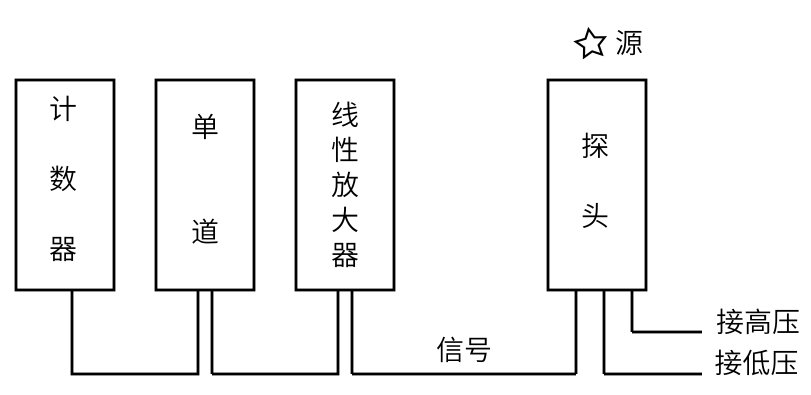
\includegraphics[width=0.45\textwidth]{lianjie.png}
\\
\xiaowu\song 图~1\begin{minipage}[t]{75mm} \quad 高压坪测试仪器连接图。单道应该工作在积分模式下,用于去除噪声。\\[-1mm]\wuhao
\end{minipage}
\end{center}

根据高压坪曲线可以选定探测器工作所应该使用的高压值。随后就可以测量探测器的能量分辨率。测量仪器示意图如下:

\begin{center}
   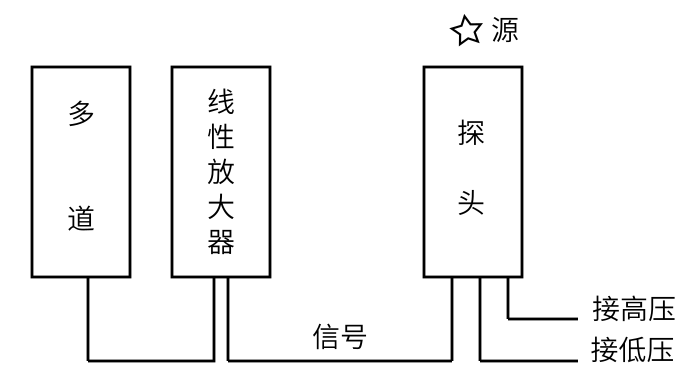
\includegraphics[width=0.45\textwidth]{lianjie2.png}
\\
\xiaowu\song 图~2\begin{minipage}[t]{75mm} \quad 探测器能量分辨率测量示意图。\\[-1mm]\wuhao
\end{minipage}
\end{center}


能量分辨率的定义为:
\begin{equation}
   R = \Delta V/V\times100\%
\end{equation}
其中$V$为测量单能射线的峰值道数,$\Delta V$则为该峰的半高宽。 

影响探测器能量分辨率因素有很多,例如在包装闪烁体的时候就应该留意包装的方式,避免有未包装的空隙。耦合时也需要选取较为光滑的闪烁体面进行耦合,避免因为划痕而造成耦合较差。

\section{实验结果和讨论}

本实验中使用的闪烁体是10号闪烁体,尺寸为底面半径为1cm,高度为4cm的圆柱体闪烁体。包装闪烁体使用的是Tyvek纸,并使其毛面接触闪烁体。实验中使用的源是$^{137}$Cs源,探测器可以探测到该源0.662MeV的全能峰,并由此测量得到探测器的能量分辨率。

本试验使用的光电倍增管为3号光电倍增管。线性放大器放大倍数为14.6倍。最终多道测量得到的数据如下图:

\begin{center}
   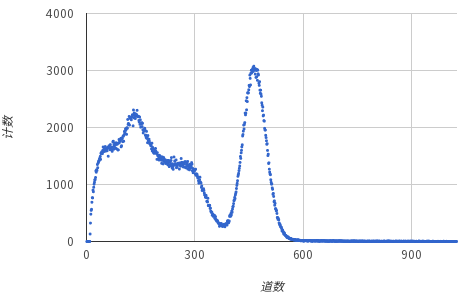
\includegraphics[width=0.45\textwidth]{jishu.png}
\\
\xiaowu\song 图~3\begin{minipage}[t]{75mm} \quad 探测器测量$^{137}$Cs能谱图。从图中可以看到源的全能峰,反散射峰以及康普顿平台。\\[-1mm]\wuhao
\end{minipage}
\end{center}

从数据图中可以得到,测量得到的Cs能谱峰值在462道处,分辨率为16\%。

因为10号仪器是新加入的,所以没有历年的数据,并不能与以往数据进行对比。但是我使用了两个不同的光电倍增管来进行测量。闪烁体,源都没有变,但是分辨率差别很大。10号光电倍增管测量得到的分辨率位18.9\%。虽然有可能是因为耦合方式带来差异,但是结合其他同学的实验结果,我觉得光电倍增管对于能量分辨率的影响更大。同时通过其他同学的测试结果得到了源的强弱并不影响探测器的能量分辨率。

\section{总结和结论}
本试验使用高4cm,半径为1cm的圆柱形CsI(Tl)闪烁体,结合光电倍增管组成探测器。最终探测器的能量分辨率为16\%。

结合其他同学的实验结果,光电倍增管的优劣对于能量分辨率的影响较大,而源的强弱对于能量分辨率基本没有影响。

\section{致谢}
感谢许金艳老师的细致地讲解以及为实验做出的准备。
\section{参考文献}

\noindent
[1] 讲义
\end{multicols}

\newpage


\section*{附录:思考题}
1、闪烁体自身的性能,包装闪烁体的材料以及包装方式,光电倍增管的性能,光电倍增管和闪烁体之间的耦合效果,电子学部分性能灯都会影响能量分辨率。

2、根据李智焕老师的课的结论,漫反射强于镜面反射。但是我觉得这个需要实验来说明。

3、耦合材料以及耦合方式直接影响到进入光电倍增管的光子数目的多少,不合理的耦合方式和材料则会使光子散失从而造成分辨率的下降。因而耦合会对分辨率产生影响

4、如果观测到的信号较为集中则分辨率好,反之则差。

5、积分和微分会影响到放大器输出的脉冲波形。因为我们使用的是多道,其直接根据脉冲高度决定道数的多少。因而微分积分时间会影响到最后多道的输出结果因而影响到能量分辨率。

6、将放射源放置在离探测器更远的地方较好,或者添加准直装置。4cm的反散射峰应该更强。

7、CsI与NaI相比,区别在于碱金属不同。两者晶体结构相近,发光原理也相近,但是Cs比Na重很多,因而与光子的反应截面也更大,所以使用CsI可以得到更好的能量分辨率。

8、不可以,分辨率太差了。区分开需要半高宽<(1.33-1.17)MeV,因而需要0.16/1.17=13.6\%的能量分辨率。因而不能分辨。
\clearpage
%\end{CJK*}
\end{document}



